\chapter{Introduction}\label{cha:1_introduction}
Recent development in networking has changed the way we think about complex systems. Researchers have concentrated their attention on a few properties that seem to be common in many real-life networks: the small-world property, power-law degree distributions and network transitivity \cite{ref-1}. One of the very challenging aspects of graphs in representing a real system is community structure. Recently, there is a growth in networks out of financial/asset transfer domains. These networks usually represent the business relationship between companies/agents. As a result, the graphs contain multiple edges between two same nodes as well as time stamps for each edge \cite{ref-19}. Analyzing the structure of a network allows us to better understand its fundamental properties by observing the characteristics and relationships between the vertices and edges of the corresponding graph. There is a growing number of distributed ledger/Blockchain-based networks that encompass the whole world and whose transaction lists are publicly accessible. Detecting community structures in massive graphs is challenging because of time and space complexity of the involved algorithms. In addition, previously identified community might change over time and might have added new transactions. Additional observation technique like birth, growth, splitting and death of communities are required to track and observe these dynamic communities \cite{ref-39}.

\section{Objectives}\label{objectives}
Finding community structures in massive networks is a growing and developing subject. The goal of this thesis is to design and develop a concept of a prototypical framework and implementation for detecting community structures and afterward observing changes in communities. The main focus of the thesis is on two complexity factors, run-time and memory management. The whole process revolves around the question "How well an approach performs on large-scale graphs?". To achieve the primary goal the following objectives had been set -
\begin{itemize}
	\item Provide an overview of state of the art community detection and observation in graphs.
	\item Conduct analysis of data sources, data types, and data concepts, preferably in the domain of Distributed Ledgers/Blockchain.
	\item Design a framework that can perform community detection and observation in large-scale transaction-based networks.
	\item Implement a prototype of the framework.
	\item Evaluate the performance (run-time and memory space requirements) of the framework.\footnote{Sample \textbf{Ethereum} data provided by SNET TU Berlin (\hyperlink{SNET-TUB}{http://www.snet.tu-berlin.de})}
\end{itemize}

This thesis focuses on the notion of community structures in blockchain network. It explores the idea that community structures exist in blockchain networks. Those community structures can be detected and monitored over time to observe the evolution of the network. For this purpose, a couple of community detection algorithm that can detect community structures in large-scale networks is tested against blockchain transaction data to determine the run-time and memory requirements. In the first chapter of this thesis, a brief introduction about communities, dynamic communities, community life-cycle, blockchain, why choosing blockchain for this thesis has been discussed. In the second chapter, an elaborate background study is discussed focusing on community detection techniques and their run-time and memory consumption. Also, the algorithms were explained in a fair manner later in chapter two. In chapter three of this thesis a prototypical framework for community structure detection and observation in large-scale network has been proposed and explained step by step. Implementation techniques and measures that has been used to test the run-time and memory consumption of the algorithms in the framework has been described in brief in chapter four. Chapter four also contains the evaluation, results and finding of the implementation. This thesis concludes with a few recommendations about future work that can be done in the field of blockchain with community detection and observation.

\section{What is a community in graph?}\label{community_in_graph}
Communities are groups of vertices which can easily be grouped together into set of nodes such that each set of node is densely connected internally and/or play similar roles within the graph \cite{ref-6}. Figure (\ref{fig:a_sample_community}) is an example of a sample graph that has three communities. Graphs representing real systems are not regular. They are objects where order coexists with disorder. The paradigm of disordered graph is the random graph \cite{ref-21}. Real networks are not random  graphs as the display big level of inhomogeneities, high level of order and organization. In real networks, the degree distribution is broad which most of the time follows power law \cite{ref-6}. As a result, many vertices with low degree coexists with some vertices with large degrees. Hence, the distribution of edges is not only globally but also locally inhomogeneous with high concentrations of edges within a special group of vertices and low concentration between these groups. This feature of real networks is called \textit{community structure} \cite{ref-1}.

\vfill
\pagebreak

\begin{figure}[H]
	\centering
	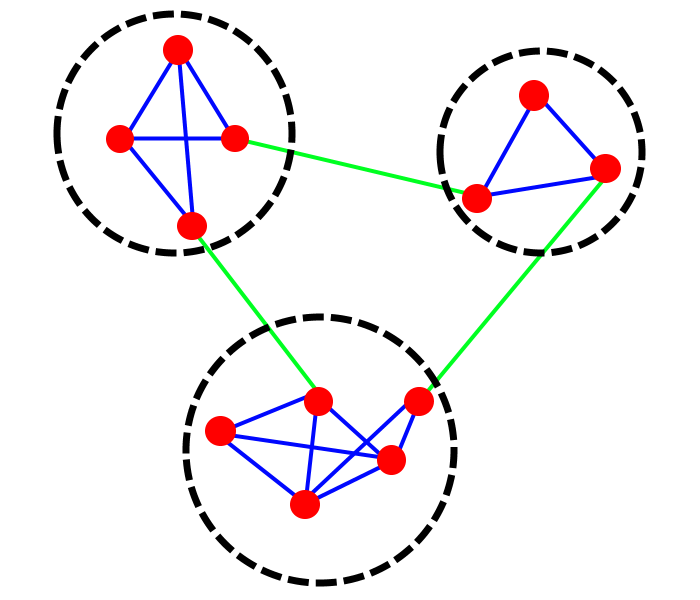
\includegraphics[width=0.5\textwidth]{community-sample}
	\caption{A graph with three communities, enclosed by dashed circles}
	\label{fig:a_sample_community}
\end{figure}

Society offers a wide range of possible groups of organizations: families, working and friendship circles, villages, towns, nations. Growth of Internet over the years also led us to the creation of virtual groups like online communities, forums and online gaming communities. Social communities have been studied for a long time \cite{ref-6}. Communities also occur in many networked systems from biology, computer science, engineering, economics, politics etc. In the graph of world wide web, they may correspond to groups of pages dealing with the same or related topics \cite{ref-36}.

Communities can have concrete applications. Clustering web clients who have similar interests and geographically near to each other may improve the performance of services provided on the world wide web, each cluster of clients can be served by a specific mirror server. Identifying clusters of customers with similar interests in the network of purchase relationship between customers and products of online retailers enables insight into customers' purchase behavior and also helps retailers to setup efficient recommendation systems \cite{ref-37}.

In every network, communities form because of some kind of interaction between nodes. In real life that could be interacting with each other. In animals that are being seen together or in a worldwide network, interaction between different system can produce community structures. In Figure (\ref{fig:communities_extra})(a), shows the famous Zachary's network of karate club members, a well-known graph regularly used in community detection benchmarking. It is consists of 34 nodes representing the 34 members of the club. It's visible from the figure that communities evolved around node 1, 33 and 34(the president of the club). The nodes in this network, inside a community is tightly connected as they represent social interaction between club members over 3 years of time period \cite{ref-58}.

Figure (\ref{fig:communities_extra})(b) shows the network of bottle-nose dolphins that were seen together more often. This also reflects the community structures in those dolphins. Figure (\ref{fig:communities_extra})(c) a relationship between AS (Autonomous Systems) form CAIDA project in 2007 is represented. It shows the interactions between different AS's. Nodes and their interactions with other AS is represented as edges and different colors represents different community structures.

\begin{figure}[H]
	\centering
	\begin{minipage}[b]{0.4\textwidth}
		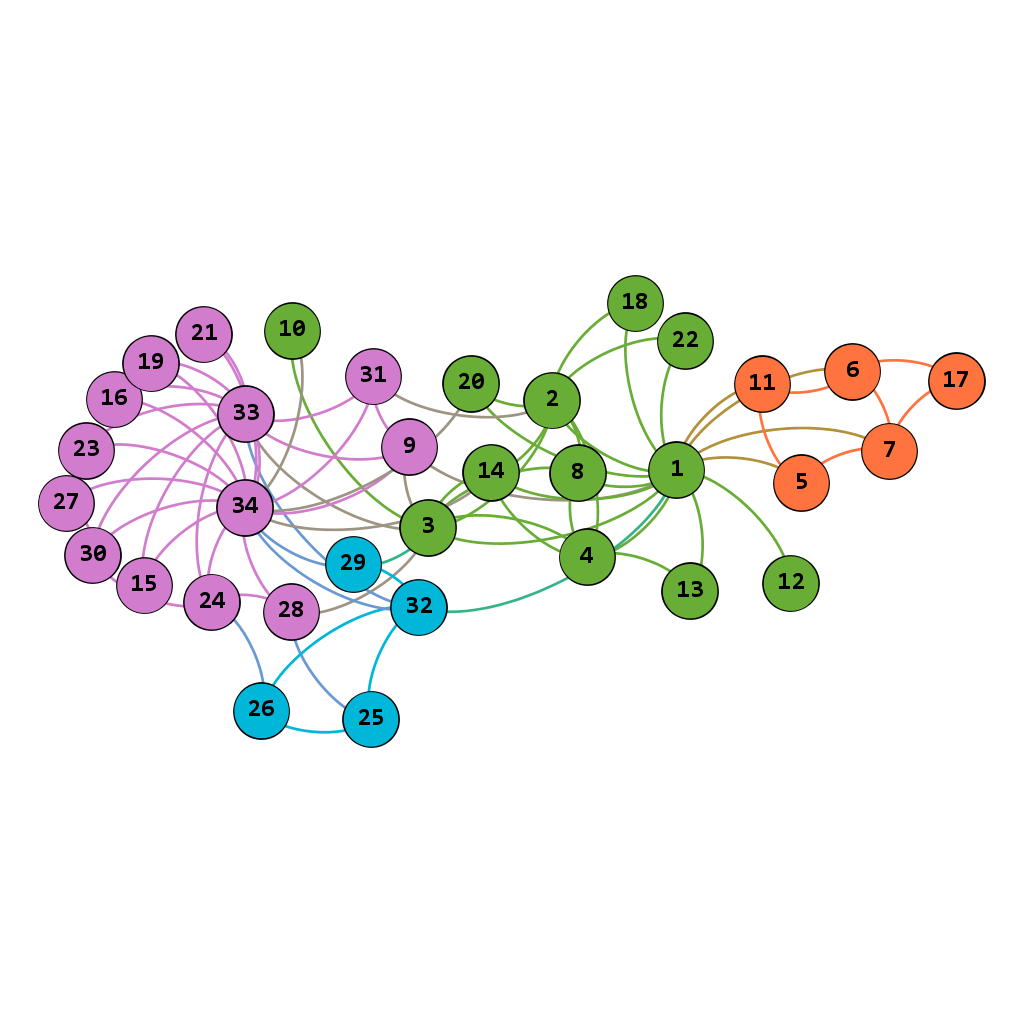
\includegraphics[width=\textwidth]{k_club_34}
		\caption*{(a)}
	\end{minipage}
	%\hfill
	\begin{minipage}[b]{0.4\textwidth}
		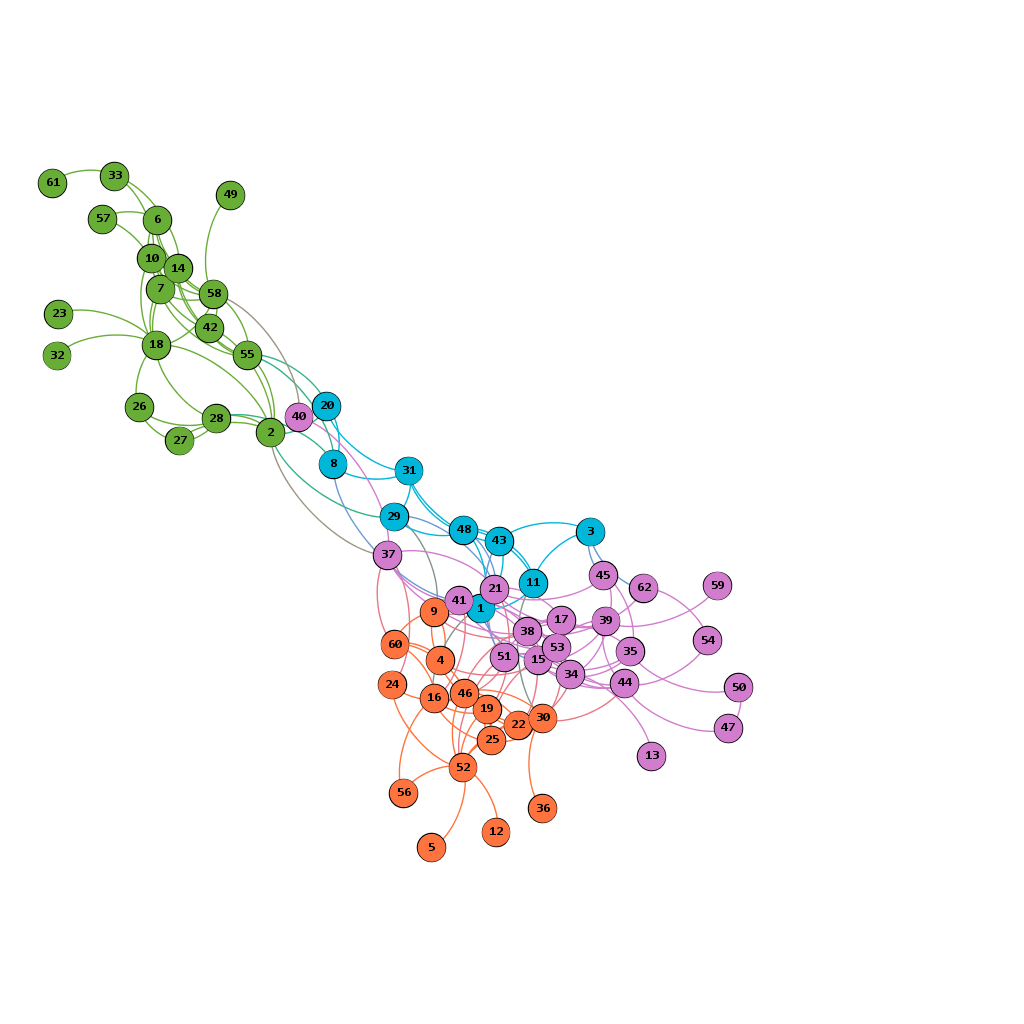
\includegraphics[width=\textwidth]{dolphins_62}
		\caption*{(b)}
	\end{minipage}
	%hfill
	\begin{minipage}[b]{0.8\textwidth}
		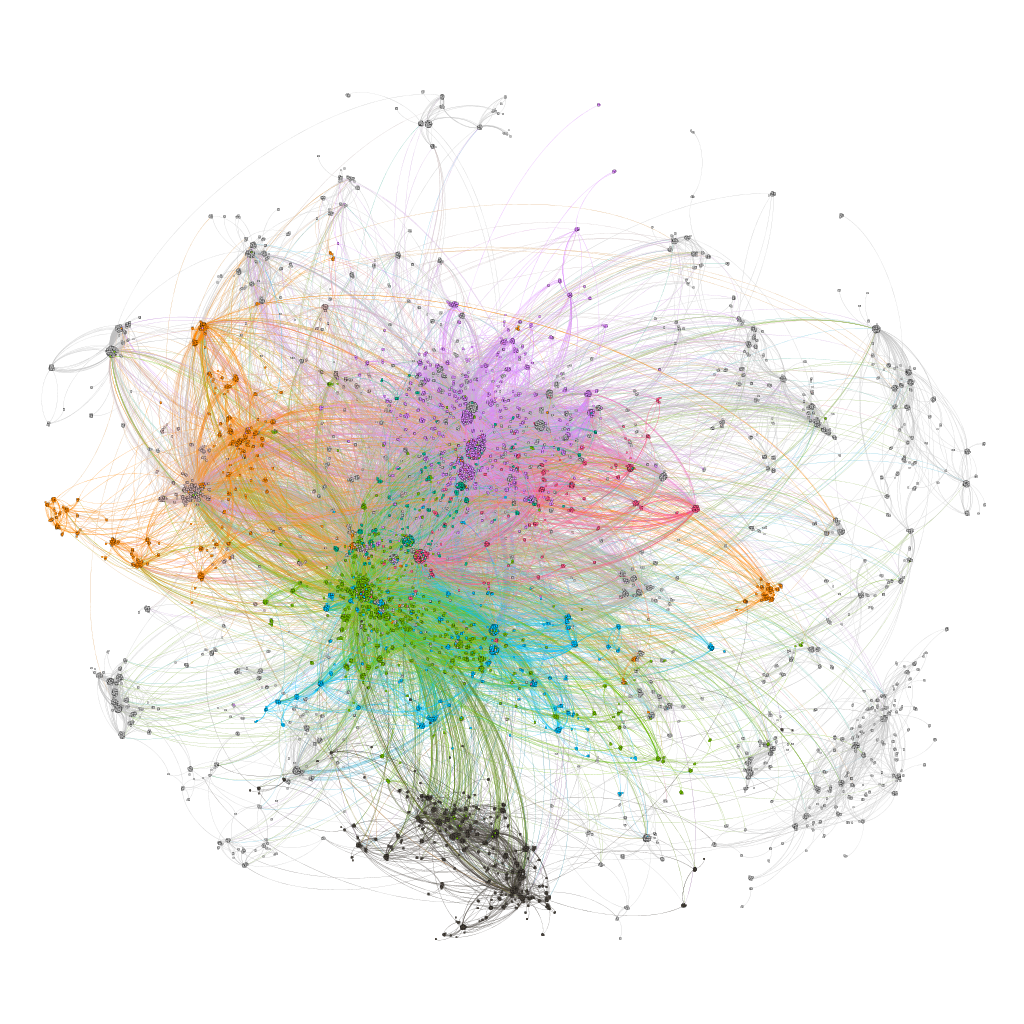
\includegraphics[width=\textwidth]{caida_26475}
		\caption*{(c)}
	\end{minipage}
	\caption{Community structures in different networks: (a) Famous Zachary's Karate club community structures. (b) Network of bottle nose dolphins (c) Community structures found in autonomous systems interaction with each other in CAIDA project in 2007}
	\label{fig:communities_extra}
\end{figure}

\section{Structure of Transaction-based Networks}
The use of network theory in transaction-based systems is relatively recent but it grew popular in the last few years. Since the data in transaction-based systems can be very different, the networks in transaction-based system are divided into similarity based networks and direct interaction networks. In similarity based networks, a link is drawn between two vertices if they share some features like strategy, behavior, income etc. This means that agents do not interact with each other but can be connected if they are similar. In direct interaction networks, a link between two nodes signals the presence of an interaction between the entities represented by the two nodes connected by the link. 

\subsection{Transaction Networks}
The most immediate application of networks to finance and economics is given whenever we have a transaction between two agents. The agents are the vertices and the transaction is the edge between them. In practice, the nodes represent banks and the weighted and directed edges represent a possible relation between banks. For transaction networks, two types of networks are considered to be most common. \textbf{First}, the inter-bank market and \textbf{Second}, payment system. Boss et al. in \cite{ref-20}, the inter-bank market is described as a network where the vertices given by the banks are nodes and the claim and liabilities between them are described as links. The inter-bank market is, therefore, a weighted and directed network.

\section{Distributed Ledger / Blockchain}
Blockchain is a distributed database solution that maintains a continuously growing list of data records that are confirmed by the nodes participating in it. Figure (\ref{fig:blockchain}) explains blockchain technology and it's different steps in the process of approving a transaction and adding a block of data to the root chain of blocks. The data is recorded in a public ledger, including information about every transaction ever completed. Blockchain is a decentralized solution which does not require any third party organization in the middle. The information about every transaction ever completed in Blockchain is shared and available to all nodes.
This attribute makes the system more transparent than centralized transactions involving a third party. In addition, the nodes in Blockchain are all pseudonymized, which makes it more secure for other nodes to confirm the transactions. Bitcoin was the first application that introduced Blockchain technology. Bitcoin created a decentralized environment for cryptocurrency, where the participants can buy and exchange goods with digital money \cite{ref-40}. A blockchain database is managed autonomously using a peer-to-peer network and a distributed time-stamping server. They are authenticated by mass collaboration powered by collective self-interests. The result is a robust work-flow where participants' uncertainty regarding data security is marginal.

\vfill
\pagebreak

\begin{figure}[H]
	\centering
	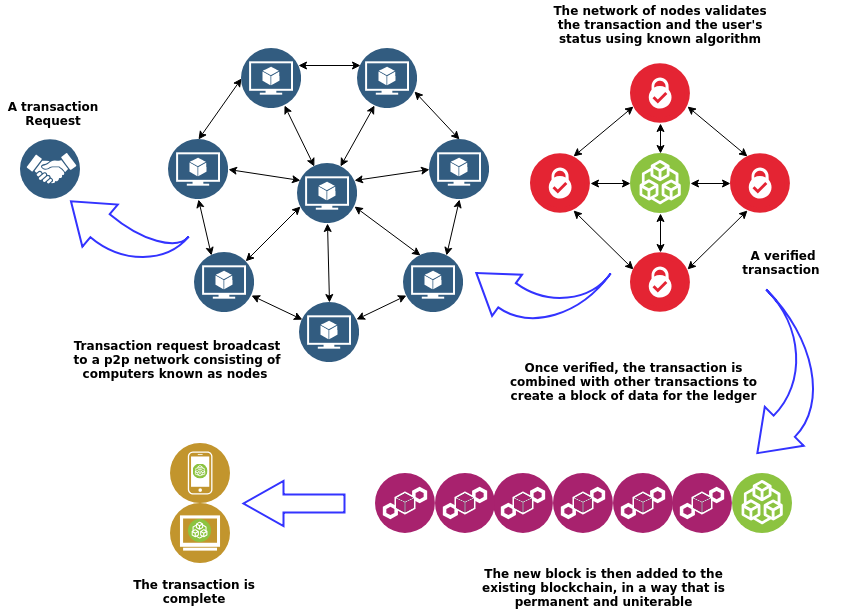
\includegraphics[width=\textwidth]{blockchain-explained}
	\caption{Blockchain explained}
	\label{fig:blockchain}
\end{figure}

\subsection{Why Blockchain?}
Blockchain is gaining popularity day by day for the past few years because of the security and anonymity it offers. Blockchain technology has allowed \textit{bitcoin} to flourish and become one of the most successful cryptocurrency over the years \cite{ref-41}. Blockchain transactions are worldwide and all the transaction data is public because it uses a distributed ledger system. It offers anonymity and irreversible, virtually unhackable security that protects transactions and assets. In Figure (\ref{fig:blockchain}), it shows that an approved block contains the hash of previous block and the previous block contains the hash it's previous block and so on. So to alter a block in the chain would be nearly impossible because to change one block, all the blocks needed to be changed and because it uses distributed ledger it's nearly impossible to get hold of all the ledger copies that are available over internet. There is also a business gain from ICO (Initial Coin Offering) from blockchain community for investing in different project. Its practically IPO (Initial Public Offering) on the basis of cryptocurrency. ICOs are changing how investors invest in and with cryptocurrency. So it's gaining popularity quick and people are getting more interested in buying cryptocurrency which leads to high value of cryptocurrency in the real world market. Blockchain technology is being used for asset transactions so it is a massive transaction-based network. For the scope of this thesis, blockchain is a suitable match as the transaction data is public, network is massive and transaction-based. Studying blockchain data and analyzing the network structure of blockchain will provide more deep insight about the properties of blockchain and network itself. It will also provide insight into business applications of blockchain. The security architecture can be better understood from blockchain through community detection and observation. It will also help to learn how the transaction-based networking is changing over time allowing us to analyze the past transactions and predict future behavior of the network itself.

\section{Community Detection in Transaction-based Networks}
Recently the research on network-based graph theories has increased \cite{ref-1}. As a result, the complex and large-scale systems are being researched as well, based on different kinds of networks that exist in real-life. So to detect communities in a large-scale transaction-based systems, it is necessary to explore the idea of community, detection of community structures in large or massive graphs representing a system, characteristics of detecting communities in large-scale networks. It might also be necessary to explore additional techniques to actively monitor and keep track of previously detected community structures in a massive graph.

\subsection{Detection of Dynamic Community}\label{subsub:dynamic_community}
Community structures can change over time in transaction-based networks. It can have new nodes and new edges in between the existing nodes or can have new nodes connected to the old nodes through new edges. Those communities are actively changing its structure over time. It's a difficult and time consuming task to keep track of constantly changing communities. The analysis of dynamic communities is still in its infancy \cite{ref-6}. Studies in this direction have been mostly hindered by the fact that the problem of graph clustering is already controversial on single graph realizations, so it is understandable that most efforts still concentrate on the \textit{static} version of the problem. Another difficulty is represented by the dearth of time-stamped data on real graphs. Recently, several data-sets have become available, enabling to monitor the evolution in time of real systems \cite{ref-23}. So it has become possible to investigate how communities form, evolve and die. The main phenomena occurring in the lifetime of a community are in Figure (\ref{fig:community_evolution}): birth, growth, contraction, merger with other communities, split, death.

\vfill
\pagebreak

\begin{figure}[!ht]
	\centering
	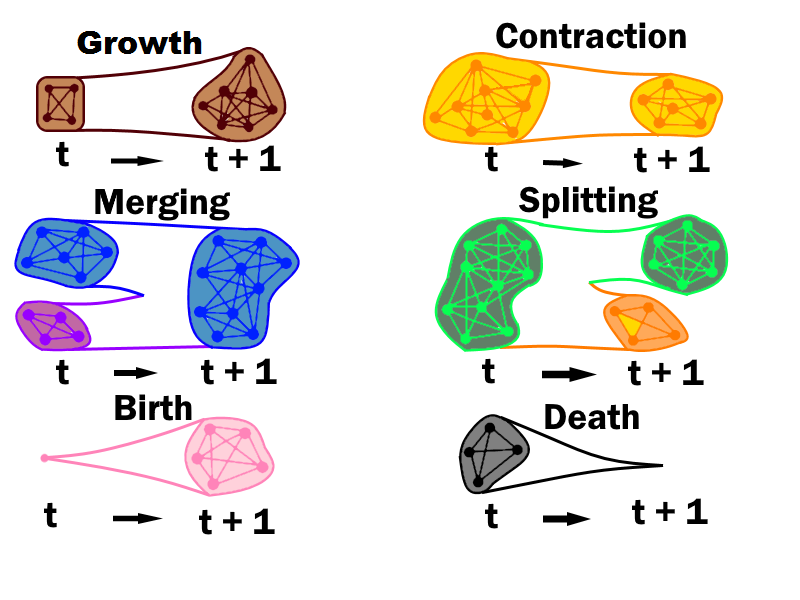
\includegraphics[width=0.7\textwidth]{community-evolution}
	\caption{Possible scenarios of community evolution \cite{ref-23}}
	\label{fig:community_evolution}
\end{figure}

One of the main objectives of this thesis is to explore and observe how community changes over the time and how to create a structured framework to track communities over time. Figure (\ref{fig:community_evolution}) is a good example of community changing over time. Community can get bigger or smaller, it can also split into different communities and can die.